\documentclass{classrep}
\usepackage{color}
\usepackage{url}
\usepackage{hyperref}
\usepackage{amsmath}
\usepackage[T1]{fontenc}
\usepackage{polski}
\usepackage[utf8]{inputenc}
\usepackage{graphicx}
\graphicspath{ {./rys/} }

\usepackage{etoolbox}
\let\bbordermatrix\bordermatrix
\patchcmd{\bbordermatrix}{8.75}{4.75}{}{}
\patchcmd{\bbordermatrix}{\left(}{\left[}{}{}
\patchcmd{\bbordermatrix}{\right)}{\right]}{}{}

\studycycle{Informatyka, studia dzienne, I st.}
\coursesemester{VI}

\coursename{Komputerowe systemy rozpoznawania}
\courseyear{2019/2020}

\courseteacher{dr inż. Marcin Kacprowicz}
\coursegroup{poniedziałek, 12:00}

\author{
  \studentinfo{Radosław Grela}{216769} \and
  \studentinfo{Jakub Wąchała}{216914} 
}

\title{Zadanie 1: ekstrakcja cech, miary podobieństwa, klasyfikacja}
\svnurl{https://github.com/Bonniu/KSR}

\begin{document}
\maketitle

\section{Cel} % Cel
Celem naszego zadania było stworzenie aplikacji do klasyfikacji tekstów za pomocą metody k-NN (k najbliższych sąsiadów) oraz
różnych metryk i miar podobieństwa, a następnie porównać kategorie z tymi wygenerowanymi przez aplikację.

\section{Wprowadzenie} % Wprowadzenie
Głównym zagadnieniem projektowym, z którym mieliśmy do czynienia w ramach zadania 1 była klasyfikacja statystyczna tekstów na podstawie wektora wyekstrahowanych cech. Do przeprowadzenie eksperymentu zaimplementowaliśmy algorytm \textsl{k-najbliższych sąsiadów}.

Algorytm k-najbliższych sąsiadów \textsl{(k-NN - k-nearest neighbors)} to jeden z algorytmów zaliczanych do grupy algorytmów leniwych. Jest to taka grupa algorytmów, która szuka rozwiązania dopiero, gdy pojawia się wzorzec testujący. Przechowuje wzorce uczące, a dopiero później wyznacza się odległość wzorca testowego względem wzorców treningowych. \cite{leniwy}. 

Algorytm ten działa w taki sposób, że dla każdego wzorca testowego obliczana jest odległość za pomocą wybranej wetryki względem wzorców treningowych, a następnie wybierana jest k najbliższych wzorców treningowych. Wynik wyznaczony jest jako najczęstszy element wśród nich. W naszym zadaniu odległość ta jest równa skali podobieństwa tekstów. 
% cechy
%Stosunek słów kluczowych do wszystkich słów w pierwszych 10% tekstu
%Stosunek słów kluczowych do wszystkich słów w ostatnich 10% tekstu
%Stosunek słów kluczowych do wszystkich słów w dokumencie
%Stosunek słów kluczowych gdzie ilość liter (0,4] do wszystkich słów
%Stosunek słów kluczowych do wszystkich słów gdzie ilość liter słów kluczowych 8+
%Stosunek linii do ilości akapitów
%Stosunek słów o długości >6 do wszystkich słów
%Stosunek słów o długości <=6 do wszystkich słów
%Ilość słów unikalnych
%Ilość słów, których długość wynosi [5,8]
\subsection{Ekstrakcja cech}
Do ekstrakcji cech charakterystycznych tekstu utworzyliśmy wektor cech, który opisuje tekst za pomocą 10 cech. Liczba słów zawsze jest liczona po zastosowaniu stop-listy oraz stemizacji, bez znaków przestankowych.
\begin{itemize}
\item[•] $C_1$ - Stosunek słów kluczowych do wszystkich słów w pierwszych 10\% tekstu. Obliczona jest za pomocą wzoru:
\begin{equation} C_1 = s_{k10} / s_{10}  \end{equation} gdzie $s_{k10}$ to liczba słów kluczowych, a $s_{10}$ to liczba wszystkich słów w pierwszych 10\% tekstu. Przed normalizacją cecha $C_{1}$ zawierała się w wartościach $\in [0,1]$.
\item[•] $C_2$ - Stosunek słów kluczowych do wszystkich słów w ostatnich 10\% tekstu. Obliczona jest za pomocą wzoru:
\begin{equation} C_2 = s_{k90} / s_{90}  \end{equation} gdzie $s_{k90}$ to liczba słów kluczowych, a $s_{90}$ to liczba wszystkich słów w ostatnich 10\% tekstu. Przed normalizacją cecha $C_{2}$ zawierała się w wartościach $\in [0,0.5]$.
\item[•] $C_3$ - Stosunek słów kluczowych do wszystkich słów w dokumencie. Obliczona jest za pomocą wzoru:
\begin{equation} C_3 = s_k / s  \end{equation} gdzie $s_k$ to liczba słów kluczowych, a $s$ to liczba wszystkich słów w dokumencie. 
Przed normalizacją cecha $C_{3}$ zawierała się w wartościach $\in [0,0.155]$.
\item[•] $C_4$ - Stosunek słów kluczowych, których ilość liter $\in$ (0,4] do wszystkich słów w dokumencie. Obliczona jest za pomocą wzoru:
\begin{equation} C_4 = s_k / s  \end{equation} gdzie $s_k$ to liczba słów kluczowych,  których ilość liter $\in$ (0,4], a $s$ to liczba wszystkich słów w dokumencie.
Przed normalizacją cecha $C_{4}$ zawierała się w wartościach $\in [0,0.075]$.
\item[•] $C_5$ - Stosunek słów kluczowych, których ilość liter jest $\geq$8 do wszystkich słów w dokumencie. Obliczona jest za pomocą wzoru:
\begin{equation} C_5 = s_k / s  \end{equation} gdzie $s_k$ to liczba słów kluczowych, a $s$ to liczba wszystkich słów w dokumencie.
Przed normalizacją cecha $C_{5}$ zawierała się w wartościach $\in [0,0.1]$.
\item[•] $C_6$ - Stosunek linii do ilości akapitów. Obliczona jest za pomocą wzoru:
\begin{equation} C_6 = l / a  \end{equation} gdzie $l$ to liczba linii, a $a$ to liczba akapitów.
Przed normalizacją cecha $C_{6}$ zawierała się w wartościach $\in [1,14]$.
\item[•] $C_7$ - Stosunek słów, których ilość liter jest większa niż 6 do wszystkich słów. Obliczona jest za pomocą wzoru:
\begin{equation} C_7 = s_6 / s  \end{equation} gdzie $s_6$ to liczba słów których ilość liter jest większa niż 6, a $s$ to liczba wszystkich słów w dokumencie.
Przed normalizacją cecha $C_{7}$ zawierała się w wartościach $\in [0,0.591]$.
\item[•] $C_8$ - Stosunek słów kluczowych, których ilość liter jest $\leq$6 do wszystkich słów w dokumencie. Obliczona jest za pomocą wzoru:
\begin{equation} C_8 = s_{6m} / s  \end{equation} gdzie $s_{6m}$ to liczba słów kluczowych, których ilość liter jest $\leq$6, a $s$ to liczba wszystkich słów w dokumencie. Przed normalizacją cecha $C_{8}$ zawierała się w wartościach $\in [0.409,1]$.
\item[•] $C_9$ - Ilość słów unikalnych. Jest to liczba słów, które wystąpiły w tekście co najmniej raz. Przykładowo, dla zdania \textsl{,,Być albo nie być''} ilość słów unikalnych jest równa 3 (\textsl{być, albo, nie}).
Przed normalizacją cecha $C_{9}$ przyjmuje wartości $\in [1,420]$.
\item[•] $C_{10}$ - Ilość słów, których ilość liter $\in$ [5,8]. Pseudokod obliczający wartość cechy $C_{10}$:
\textsl{
\begin{itemize}
\item $C_{10}$=0
\item Dla każdego słowa w artykule:
	\begin{itemize}
	\item Jeżeli długość słowa>=5 i długość słowa <=8:
		\begin{itemize}
		\item $C_{10}$++;
		\end{itemize}
	\end{itemize}
\item Zwróć $C_{10}$
\end{itemize}
} 
Przed normalizacją cecha $C_{10}$ zawierała się w wartościach $\in [1,574]$.
\end{itemize}
{\color{blue}
- W przypadku cech mniej intuicyjnych (a najlepiej wszystkich) - mile widziany przykład jak liczyć (może być jeden tekst dla wszystkich cech pod ich opisem).
- Jakie znaczenie ma ta cecha tekstu dla jego rozpoznania? Czy np. im tekst dłuższy, tym bardziej związany z etykietą USA lub CANADA? (istotne!)}
\subsection{Metryki i miary}
Do liczenia odległości pomiędzy artykułami oraz obliczenia miary podobieństwa używaliśmy 3 metryk i 2 miar.
\begin{enumerate}
\item Metryka Euklidesowa - aby obliczyć odległość $d_e(x,y)$ między artykułami x i y należy obliczyć pierwiastek kwadratowy z sumy kwadratów różnic wartości współrzędnych wektora o tych samych indeksach. Wzór jest następujący:
\begin{equation} 
d_e(x,y)=\sqrt{(x_1-y_1)^2+\ldots+(x_n-y_n)^2}
\end{equation}
\item Metryka Manhattan - odległość $d_m(x,y)$ jest równa sumie wartości bezwzględnych z różnic wartości współrzędnych wektora o tych samych indeksach:
\begin{equation} 
d_m(x,y)=\sum_{n=1}^{N} |{x_n-y_n}|
\end{equation}
\item Metryka Czebyszewa - odległość $d_c(x,y)$ w tej metryce jest równa maksymalnej wartości bezwględnych różnic współrzędnych punktów x oraz y, zgodnie ze wzorem:
\begin{equation} 
d_c(x,y)=\max_{i} |{x_i-y_i}|
\end{equation}
\item Miara \textsl{Term Frequency Matrix}, czyli po polsku ,,macierz częstości występowania terminów'' podaje wartość podobieństwa dokumentów $d_1$ i $d_2$ ze względu na wybrany zbiór terminów, np. słów kluczowych. Ustawiamy macierz słów kluczowych i dokumentów:
\begin{equation}
\bbordermatrix{~ & t_1 & t_2 & \ldots & t_n \cr
                  d_1 & a_{11} & a_{12} & \ldots & a_{1n} \cr
                  d_2 & a_{21} & a_{22} & \ldots & a_{2n} \cr}
\end{equation}
Następnie podobieństwo otrzymanych wektorów jest obliczone przy pomocy amplitudy kosinusowej: 
\begin{equation}
r_{ca}(V_1, V_2)= \textsl{$\frac{|\sum_{i=1}^{n} a_{1i}*a_{2i}|}{\sqrt{\sum_{i=1}^{n} a_{1i}^2 * \sum_{i=1}^{n} a_{2i}^2}}$}
\end{equation}
\item Miara \textsl{n-gramów} 

%\item Odległość Minkowskiego \cite{wyklad} - jest to uogólniony wzór odległości euklidesowej, miejskiej oraz Czebyszewa. Odległość
%$L_m(x,y)$ w tej metryce dla m=3, zgodnie ze wzorem jest równa \cite{minkowski}:
%\begin{equation} 
%L_m(x,y)=\sqrt[m]{|x_1-y_1|^m+\ldots+|x_n-y_n|^m}
%\end{equation}
%Dla m=3, czyli parametru użytego w naszym programie:
%\begin{equation} 
%L_3(x,y)=\sqrt[3]{|x_1-y_1|^3+\ldots+|x_n-y_n|^3}
%\end{equation}
%\item \textsl{Canberra distance} \cite{wyklad} - odległość $d_{can}(x,y)$ w tej metryce jest równa sumie ilorazów wartości bezwględnej %różnicy współrzędnych wektorów x oraz y z sumą wartości bezwzględnych współrzędnych wektorów x oraz y, zgodnie ze wzorem: %\cite{canberra}
%\begin{equation} 
%d_{can}(x,y)=\sum_{n=1}^{N} \frac{|x_n-y_n|}{|x_n|+|y_n|}
%\end{equation}

\end{enumerate}





\section{Opis implementacji} % Opis implementacji
{\color{blue}
Należy tu zamieścić krótki i zwięzły opis zaprojektowanych klas oraz powiązań
między nimi. Powinien się tu również znaleźć diagram UML  (diagram klas)
prezentujący najistotniejsze elementy stworzonej aplikacji. Należy także
podać, w jakim języku programowania została stworzona aplikacja. }

\section{Materiały i metody} % Materiały i metody
Wykonana przez nas klasyfikacja została wykonana za pomocą wszystkich trzech metryk. Każdy przypadek testowy był klasyfikowany dla dziesięciu różnych wartości k najbliższych sąsiadów: 2, 3, 4, 5, 7, 10, 13, 15, 20, 25.

Klasyfikacji dokonywaliśmy tylko na tych tekstach, które miały jedną z etykiet: \textsl{west-germany, usa, france, uk, canada, japan} i były to ich jedyne etykiety.

Dokonaliśmy pięciu różnych podziałów na dane testowe oraz treningowe:
\begin{itemize}
\item 10\% dane treningowe, 90\% dane testowe
\item 30\% dane treningowe, 70\% dane testowe
\item 50\% dane treningowe, 50\% dane testowe
\item 70\% dane treningowe, 30\% dane testowe
\item 85\% dane treningowe, 15\% dane testowe
\end{itemize}

\newpage
\section{Wyniki} % Wyniki
\subsection{Badanie podziału na dane treningowe i testowe}

\begin{table}[h!]
	\centering
	\begin{tabular} {c c}
		\hline
		\textbf{k} & \textbf{Accuracy [\%]} \\ [0.5ex] 
		\hline
		\hline 
		2 & 66,19 \\ 
		3 & 72,61 \\
		4 & 73,81 \\
		5 & 75,87 \\
		7 & 77,56 \\
		10 & 77,95  \\
		13 & 78,71 \\ 
		15 & 78,98 \\
		20 & 79,07 \\
		25 & 79,41 \\
		\hline
	\end{tabular}
	\caption{Skuteczność klasyfikacji dla metryki Euklidesowej dla podziału zbioru 30\% treningowe/70\% testowe. }
\end{table}

\begin{table}[h!]
	\centering
	\begin{tabular} {c c}
		\hline
		\textbf{k} & \textbf{Accuracy [\%]} \\ [0.5ex] 
		\hline
		\hline 
		2 & 67,14 \\ 
		3 & 72,97 \\
		4 & 74,25 \\
		5 & 75,79 \\
		7 & 77,82 \\
		10 & 78,74  \\
		13 & 79,26 \\ 
		15 & 79,35 \\
		20 & 79,74 \\
		25 & 79,81 \\
		\hline
	\end{tabular}
	\caption{Skuteczność klasyfikacji dla metryki Euklidesowej dla podziału zbioru 50\% treningowe/50\% testowe. }
\end{table}

\begin{table}[h!]
	\centering
	\begin{tabular} {c c}
		\hline
		\textbf{k} &\textbf{Accuracy [\%]} \\ [0.5ex] 
		\hline
		\hline 
		2 & 67,62 \\ 
		3 & 73,95 \\
		4 & 75,52 \\
		5 & 77,64 \\
		7 & 79,86 \\
		10 & 80,77  \\
		13 & 81,11 \\ 
		15 & 81,38 \\
		20 & 81,38 \\
		25 & 81,48 \\
		\hline
	\end{tabular}
	\caption{Skuteczność klasyfikacji dla metryki Euklidesowej dla podziału zbioru 70\% treningowe/30\% testowe. }
\end{table}

\begin{table}[h!]
	\centering
	\begin{tabular} {c c}
		\hline
		\textbf{k} & \textbf{Accuracy [\%]} \\ [0.5ex] 
		\hline
		\hline 
		2 & 70,56 \\ 
		3 & 76,11 \\
		4 & 77,47 \\
		5 & 79,31 \\
		7 & 81,62 \\
		10 & 82,10  \\
		13 & 82,73 \\ 
		15 & 82,80 \\
		20 & 83,17 \\
		25 & 83,09 \\
		\hline
	\end{tabular}
	\caption{Skuteczność klasyfikacji dla metryki Euklidesowej dla podziału zbioru 80\% treningowe/20\% testowe. }
\end{table}

\begin{table}[h!]
	\centering
	\begin{tabular} {c c}
		\hline
		\textbf{k} & \textbf{Accuracy [\%]} \\ [0.5ex] 
		\hline
		\hline 
		2 & 72,16 \\ 
		3 & 76,99 \\
		4 & 78,60 \\
		5 & 80,16 \\
		7 & 82,59 \\
		10 & 83,13  \\
		13 & 83,67 \\ 
		15 & 83,72 \\
		20 & 84,06 \\
		25 & 84,30 \\
		\hline
	\end{tabular}
	\caption{Skuteczność klasyfikacji dla metryki Euklidesowej dla podziału zbioru 85\% treningowe/15\% testowe. }
\end{table}

\begin{figure}[h!]
    \centering
    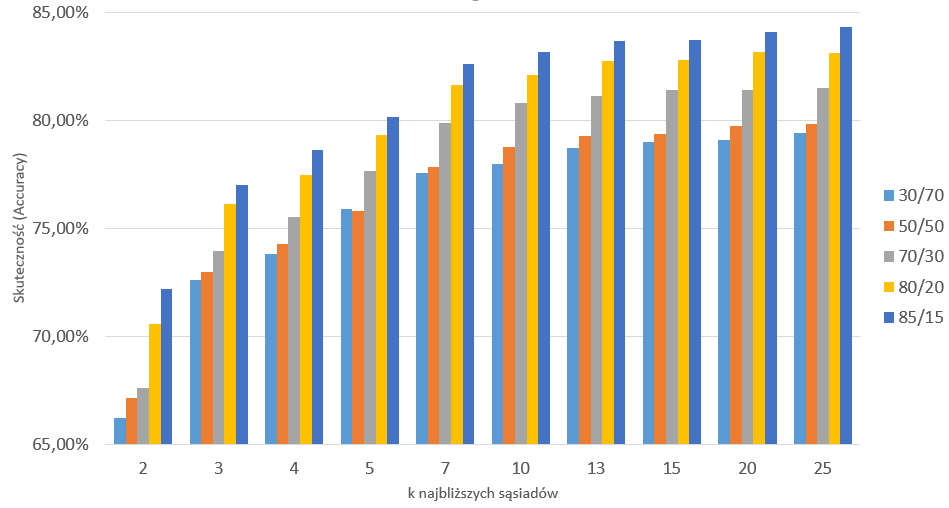
\includegraphics[width=1\textwidth]{testtren.png}
    \caption{Dane z tabel 1-5 zebrane na wykresie.}
    \label{testtren}
\end{figure}

\begin{table}[h!]
	\centering
	\begin{tabular} {c c}
		\hline
		\textbf{Dane treningowe/testowe} & \textbf{Accuracy [\%]} \\ [0.5ex] 
		\hline
		\hline 
		30/70 & 77,95 \\ 
		50/50 & 78,74 \\
		70/30 & 80,77 \\
		80/20 & 82,10 \\
		85/15 & 83,13 \\
		\hline
	\end{tabular}
	\caption{Zależność Accuracy od pięciu wartości proporcji podziału zbioru dla k=10. }
\end{table}

\begin{figure}[h!]
    \centering
    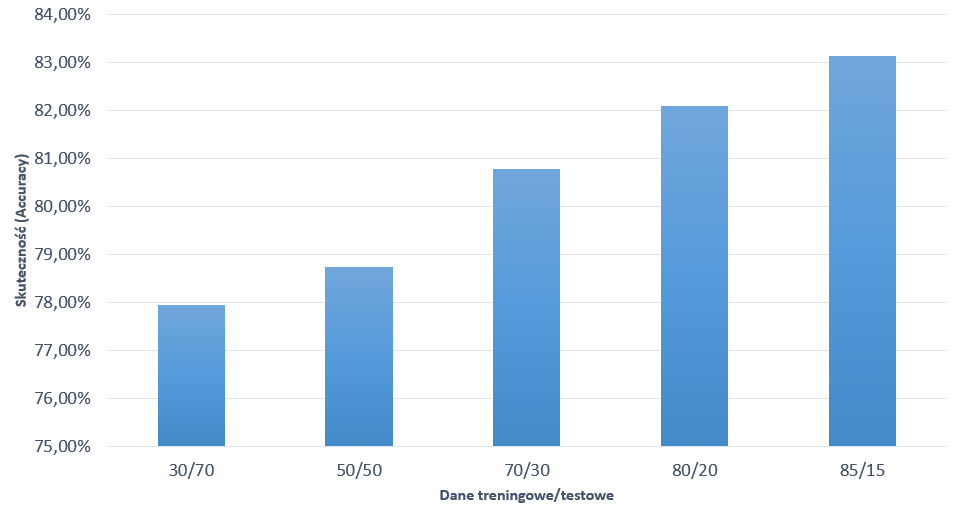
\includegraphics[width=1\textwidth]{5podzialk10.png}
    \caption{Wykres przedstawiający zależność Accuracy od pięciu wartości proporcji podziału zbioru dla k=10.}
    \label{5podzialk10}
\end{figure}

\begin{table}[h!]
	\centering
	\begin{tabular} {c c}
		\hline
		\textbf{Metryka} & \textbf{Accuracy [\%]} \\ [0.5ex] 
		\hline
		\hline 
		Eulkidesowa & 77,82 \\ 
		Czebyszewa & 78,18 \\
		Manhattan &77,72 \\
		\hline
	\end{tabular}
	\caption{Zależność Accuracy od wyboru metryki dla k=7 i podziału 50/50. }
\end{table}

\begin{figure}[h!]
    \centering
    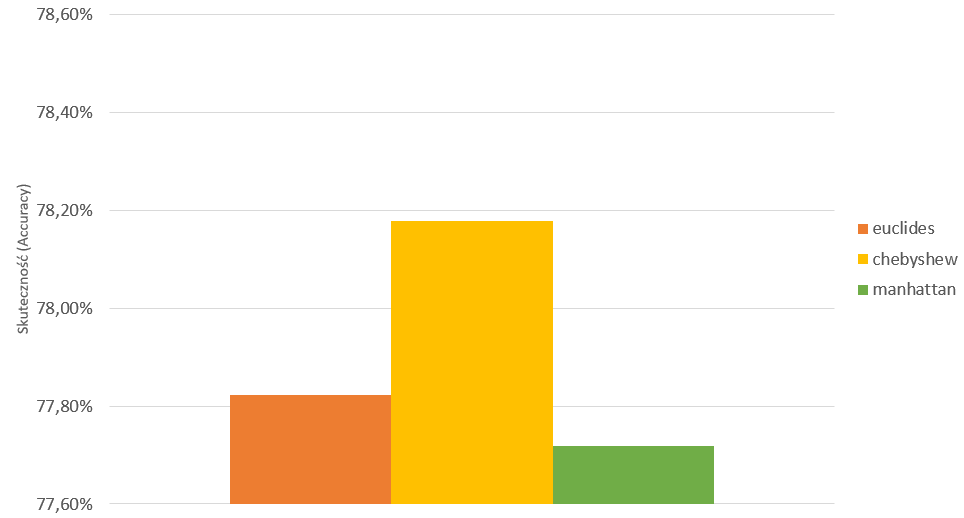
\includegraphics[width=1\textwidth]{metryki.png}
    \caption{Wykres przedstawiający zależność Accuracy od wyboru metryki dla k=7 i podziału 50/50.}
    \label{metryki}
\end{figure}

\newpage
\section{Dyskusja} % Dyskusja
{\color{blue}
Sekcja ta powinna zawierać dokładną interpretację uzyskanych wyników
eksperymentów wraz ze szczegółowymi wnioskami z nich płynącymi. Najcenniejsze
są, rzecz jasna, wnioski o charakterze uniwersalnym, które mogą być istotne
przy innych, podobnych zadaniach. Należy również omówić i wyjaśnić wszystkie
napotakane problemy (jeśli takie były). Każdy wniosek powinien mieć poparcie
we wcześniej przeprowadzonych eksperymentach (odwołania do konkretnych
wyników). Jest to jedna z najważniejszych sekcji tego sprawozdania, gdyż
prezentuje poziom zrozumienia badanego problemu.}
\section{Wnioski}
{\color{blue}W tej, przedostatniej, sekcji należy zamieścić podsumowanie
najważniejszych wniosków z sekcji poprzedniej. Najlepiej jest je po prostu
wypunktować. Znów, tak jak poprzednio, najistotniejsze są wnioski o
charakterze uniwersalnym.}


\begin{thebibliography} {0}
\bibitem{leniwy} \textsl{http://home.agh.edu.pl/~horzyk/lectures/miw/KNN.pdf} [dostęp 22.03.2020]
\bibitem{minkowski} \textsl{https://pl.wikipedia.org/wiki/Odleg\%C5\%82o\%C5\%9B\%C4\%87\_Minkowskiego} [dostęp 22.03.2020]
\bibitem{canberra} \textsl{https://en.wikipedia.org/wiki/Canberra\_distance} [dostęp 22.03.2020]
\bibitem{wyklad} \textsl{https://ftims.edu.p.lodz.pl/pluginfile.php/132368/mod\_folder/content/0/
ksr-wyklad-2009.pdf?forcedownload=1} [dostęp 22.03.2020]
\end{thebibliography}
\end{document}
